\section*{Problems}

\subsection*{Multiple-Choice Questions}
\begin{multicols}{2}
  \begin{enumerate}[itemsep=6pt,leftmargin=15pt]

  \item A car moves in a horizontal circle with a radius of \SI{10}\metre. The
    tangential velocity of the car is \SI{30}{\metre\per\second}. What is the
    car's acceleration?
    \begin{enumerate}
    \item\SI3{\metre\per\second\squared} towards the centre
    \item\SI3{\metre\per\second\squared} away from the centre
    \item\SI{90}{\metre\per\second\squared} towards the centre
    \item\SI{90}{\metre\per\second\squared} away from the centre
    \item\SI{270}{\metre\per\second\squared} towards the centre
    \end{enumerate}
  
  \item If the car in the previous question has a mass of
    \SI{1000}{\kilo\gram}, what is the force of friction acting on the car?
    \begin{enumerate}
    \item\SI{3000}{\newton} towards the centre
    \item\SI{3000}{\newton} away from the centre
    \item\SI{90000}{\newton} away from the centre
    \item\SI{90000}{\newton} towards the centre
    \item\SI{90000}{\newton} vertically
    \end{enumerate}
  
  \item A \SI{1000}{\kilo\gram} car experiences a centripetal force of
    \SI{1.8e5}{\newton} while making a turn. The car is moving at a constant
    speed of \SI{30}{\metre\per\second}. What is the radius of the turn?
    \begin{enumerate}
    \item\SI{.2}\metre
    \item\SI1\metre
    \item\SI2\metre
    \item\SI4\metre
    \item\SI5\metre
    \end{enumerate}

  \item Friction allows a car to make a turn at a speed of 10 miles per
    hour. By what factor will the friction have to change to allow the driver to
    make the same turn at twice the speed?
    \begin{enumerate}
    \item Four times the friction
    \item Twice the friction
    \item The same amount of friction
    \item One-half the friction
    \item One-fourth the friction
    \end{enumerate}
  
  \item A tetherball is whirled in a horizontal circle above your head. If
    the string breaks, the ball will follow what type of path if it is observed
    from above?
    \begin{enumerate}
    \item Straight outward from the centre
    \item Straight towards the centre
    \item An expanding spiral
    \item A curved path that gradually approaches a straight line
    \item Tangent to the original circular path
  \end{enumerate}
  
  \item A pendulum bob is attached to a string that is tied to the ceiling,
    and the bob is pulled back and released. As the bob moves through the bottom
    of the swing, how does the magnitude of the tension force from the string
    compare to the gravitational force on the bob?
    \begin{enumerate}
    \item The tension force is less than the gravitational force.
    \item The tension force is greater than the gravitational force.
    \item The tension force is equal to the gravitational force.
    \item The mass of the ball is needed in order to compare these forces.
    \item The release height of the ball is needed in order to compare these
      forces.
    \end{enumerate}
    
  \item A ball is attached to a string and whirled in a vertical circle. The
    tension in the string will be the least
    \begin{enumerate}
    \item at the bottom of the circle
    \item at the top of the circle
    \item as the ball is moving towards the top of the circle
    \item as the ball is moving towards the bottom of the circle
    \item Trick question! Tension will be the same at all points in the circle.
    \end{enumerate}

  \item A girl stands on a rotating merry-go-round without holding on to a rail.
    The force that keeps her moving in a circle is the
    \begin{enumerate}
    \item frictional force on the girl directed away from the centre of
      the merry-go-round
    \item frictional force on the girl directed towards the centre of the
      merry-go-round
    \item normal force on the girl directed away from the centre of the
      merry-go-round
    \item normal force on the girl directed towards the centre of the
      merry-go-round
    \item weight of the girl
    \end{enumerate}
  
  \item A bicycle wheel has a radius of 0.5 m. When it spins, it completes
    one full turn in 1.6 s. A pebble wedged in the tread has a mass of 10 g.
    What is the centripetal force on the pebble?
    \begin{enumerate}
    \item\SI{.01}\newton
    \item\SI{.08}\newton
    \item\SI{.1}\newton
    \item\SI{.8}\newton
    \item\SI1\newton
    \end{enumerate}
  
  \item A tetherball swings in a horizontal circle. If the radius of the
    swing is tripled but the tangential speed remains the same, by what factor
    does the centripetal force change?
    \begin{enumerate}
    \item Nine times greater
    \item Three times greater
    \item Remains the same
    \item One-third as much
    \item One-ninth as much
    \end{enumerate}
  
  \item A car of mass $m$ drives on a flat circular track of radius $R$. To
    maintain a constant speed $v$ on the track, the coefficient of friction
    $\mu$ between the tires and the road must be
    \begin{enumerate}
    \item $mg$
    \item $mg+\dfrac{mv^2}R$
    \item $mg-\dfrac{mv^2}R$
    \item $\dfrac{v^2}{gR}$
    \item $\sqrt{\dfrac{v^2}{gR}}$
    \end{enumerate}

%  \item A car travels on a circular track that is banked at an angle
%  $\theta$ from the horizontal, as shown in the diagram below. Which of the
%  following diagrams best shows the forces acting on the car as it moves on the
%  banked track?
%  \begin{center}
%    \vspace{-.1in}
%    \pic{.18}{../graphics/banked-turn-acceleration}
%  \end{center}
%
%  \vspace{-.15in}
%  A.\begin{tikzpicture}
%    \fill circle (.08);
%    \draw[vectors] (0,0)--(0,1) node[above]{$\vec N$};
%    \draw[vectors] (0,0)--(0,-1) node[below]{$m\vec g$};
%    \draw[vectors,rotate=60] (0,0)--(0,1) node[left]{$\vec F_s$};
%  \end{tikzpicture}
%  \hspace{.2in}
%  B.\begin{tikzpicture}
%    \fill circle (.08);
%    \draw[vectors,rotate=-30] (0,0)--(0,1) node[above]{$\vec N$};
%    \draw[vectors,rotate=-30] (0,0)--(0,-1) node[below]{$m\vec g$};
%    \draw[vectors,rotate=60] (0,0)--(0,-1) node[right]{$\vec F_s$};
%  \end{tikzpicture}
%  \hspace{.2in}
%  C.\begin{tikzpicture}
%    \fill circle (.08);
%    \draw[vectors,rotate=-30] (0,0)--(0,1) node[above]{$\vec N$};
%    \draw[vectors] (0,0)--(0,-1) node[below]{$m\vec g$};
%    \draw[vectors,rotate=60] (0,0)--(0,-1) node[right]{$\vec F_s$};
%  \end{tikzpicture}
%  \hspace{.2in}
%  D.\begin{tikzpicture}
%    \fill circle (.08);
%    \draw[vectors] (0,0)--(0,1) node[above]{$\vec N$};
%    \draw[vectors] (0,0)--(0,-1) node[below]{$m\vec g$};
%    \draw[vectors,rotate=60] (0,0)--(0,-1) node[right]{$\vec F_s$};
%  \end{tikzpicture}
%  \hspace{.2in}
%  E. \begin{tikzpicture}
%    \fill circle (.08);
%    \draw[vectors,rotate=120] (0,0)--(0,1) node[left]{$\vec N$};
%    \draw[vectors] (0,0)--(0,-1) node[below]{$m\vec g$};
%    \draw[vectors,rotate=60] (0,0)--(0,-1) node[right]{$\vec F_s$};
%  \end{tikzpicture}
%  
%  \item In the previous question, which of the following statements is true
%  of the forces acting on the car while on the circular track?
%  \begin{enumerate}
%    \item The normal force the track exerts on the car provides the
%    centripetal force.
%    \item The weight of the car provides the centripetal force.
%    \item The frictional force the track exerts on the car provides the
%    centripetal force.
%    \item The centripetal force is provided by a combination of the normal
%    force and frictional force.
%    \item There is no centripetal force in this case.
    %  \end{enumerate}
  \end{enumerate}
\end{multicols}

\subsection*{Short-Answer Questions}
\begin{enumerate}[itemsep=6pt,leftmargin=15pt]
\item When drawing free-body diagrams, does the label ``centripetal
  force'' get used? Explain.
\end{enumerate}

\subsection*{Problem-Solving Questions}
\begin{enumerate}[itemsep=6pt,leftmargin=15pt]
\item A car exits a highway on a ramp that is banked at \ang{15} with a radius
  of curvature of \SI{65}\metre. If the ramp is extremely icy and the driver
  cannot depend on any friction to help make the turn, what is the safe speed
  that the driver can travel so that the car will not skid off the ramp? 
  
\item A highway curve with a radius of curvature of \SI{155}{\metre} must
  accommodate cars travelling at \SI{50}{\kilo\metre\per\hour} without
  friction. At what angle should the curve be banked? (Be careful with unit
  conversion.)

\item A pilot of mass \SI{68.5}{\kilo\gram} in a jet aircraft makes a complete
  vertical circle in mid-air. The vertical circle has a radius of
  \SI{1.70}{\kilo\metre}. The speed of the jet is \SI{215}{\metre\per\second}.
  Draw a free-body diagram of the forces acting on the pilot, determine the
  force of the seat on the pilot at
  \begin{enumerate}[itemsep=3pt]
  \item the bottom of the loop and
  \item the top of the loop
  \end{enumerate}
  (Note that at the top of the loop, the aircraft is upside down.)

  \begin{center}
    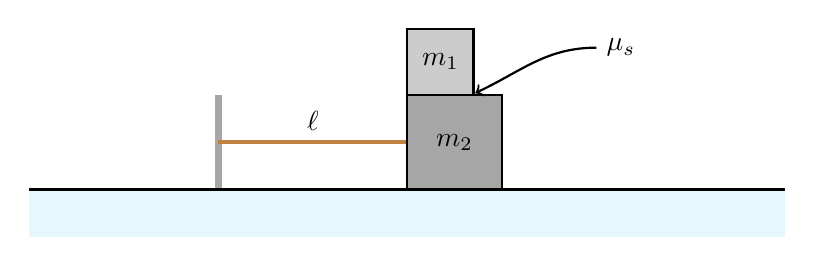
\begin{tikzpicture}[scale=1.2]
      \fill[cyan!10] rectangle (8,-.5);
      \draw[gray!70,line width=2.5] (2,0)--(2,1);
      \draw[brown,ultra thick] (2,.5)--(4,.5) node[midway,above,black]{$\ell$};
      \draw[thick,fill=gray!70] (4,0) rectangle +(1,1) node[midway]{$m_2$};
      \draw[thick,fill=gray!40] (4,1) rectangle +(.7,.7) node[midway]{$m_1$};
      \draw[very thick] (0,0)--(8,0);
      \draw[<-,thick] (4.72,1.02) to[out=25,in=180](6,1.5) node[right]{$\mu_s$};
    \end{tikzpicture}
  \end{center}
\item Mass $m_1$ (\SI{2.0}{\kilo\gram}) sits on top of mass $m_2$
  (\SI{5.0}{\kilo\gram}), which rests on a frictionless table, as shown above.
  The coefficient of static friction between the two masses is $\mu_s=0.30$. A
  string of length $\ell=\SI{5.0}\metre$ is tied to $m_2$, and both masses
  are swung around without slipping in a horizontal circle.
  \begin{enumerate}[itemsep=3pt]
  \item On two clearly labelled free-body diagrams, 
    %On the dots below,
    draw and label all the forces (not components) that act on the masses.
    Forces should be drawn as arrows originating at, and pointing away from,
    the dots that represent the masses. (Hint: There are normal forces at
    \emph{all} contacts surfaces.)%between the masses and the table.)
    %\begin{center}
    %  \begin{tikzpicture}
    %    \fill circle (.1) node[left]{$m_1$};
    %    \fill (7,0) circle (.1) node[left]{$m_2$};
    %  \end{tikzpicture}
    %\end{center}

  \item Calculate the maximum centripetal acceleration of the masses. (Hint:
    This is a multi-body problem like the stacked-body example studied in Class
    2, except in this case, we are solving for the maximum \emph{centripetal}
    acceleration. The top mass $m_1$ accelerates because of static friction.)
    
  \item Calculate the maximum speed of the masses. (Once you have the
    centripetal acceleration, this should be very simple.)
    
  \item Calculate the tension in the string when the masses are moving at
    maximum speed.
  \end{enumerate}
  
  \begin{center}
    \pic{.5}{circularMotion/graphics/twoblocks}
  \end{center}
  
\item A block of mass $m_1$ is attached to a cord of length $L_1$, which
  is fixed at one end. The mass moves in a horizontal circle supported by a
  frictionless table. A second block of mass $m_2$ is attached to the first by
  a cord of length $L_2$ and also moves in a circle, as shown in the diagram.
  If the period of the motion is $T$:
  \begin{enumerate}[itemsep=3pt]
  \item On the dots below, draw and label all the forces (not components) that
    act on the blocks. Forces should be drawn as arrows originating at, and
    pointing away from, the dots that represent the blocks.
    %\begin{center}
    %  \vspace{1in}
    %  \begin{tikzpicture}
    %    \fill circle (.1) node[left]{$m_1$};
    %    \fill (7,0) circle (.1) node[left]{$m_2$};
    %  \end{tikzpicture}
    %  \vspace{1in}
    %\end{center}    
  \item Find the tension in each cord.
  \end{enumerate}

\item\textbf{Challenge question:} In Example \ref{example:yoyo}, we have found
  the tension force on th yo-yo at the top, side and bottom of its circular
  motion. Between these points, the centripetal and tangential forces are
  provided by a combination of tension and gravitational forces.
  \begin{enumerate}[itemsep=3pt]
  \item Find the tangential force ($F_t$) as a function of $\theta$.
  \item Find the tension force ($F_t$) as a function of $\theta$.
  \end{enumerate}
\end{enumerate}


